Moving forward, there are several improvements that can be made to the 2D/1D scheme with regard to the cusping problem.  Four of these improvements will be discussed in this section.  The first two are modifications to methods already in MPACT, while the second two would involve implementation of new solvers.

\section{Improvements to Current Decusping Techniques}

The sub-plane--based decusping solvers presented in chapters \ref{chap:cusping}-\ref{chap:results} are capable of reducing the cusping errors significantly over having no treatment.  They also provide a more general solution to the problem than the polynomial corrections that existed in MPACT previously.  However, there are at least two improvements that can be made going forward.  The first deals with approximations made in the calculation of the radial currents, and the second deals with the auxiliary solver used to generate the radial flux profiles.

\subsection{Radial Transverse Leakage Source}

The current implementation of the sub-plane scheme assumes the same $\hat{D}$ current correction term for all sub-plane surfaces between two pin cells.  This assumption is made to improve the stability of the sub-plane scheme, but certainly introduces some error in the CMFD and SP$_3$ calculations.  In most cases, this error is likely quite small, since the axial shape of the solution usually changes gradually.  However, when a control rod is partially inserted into an MOC plane, the currents in the rodded sub-planes are much different from those in the unrodded sub-plane.  The CMFD calculations predict that this is the case, but using the same $\hat{D}$ for both of these regions likely introduces a more significant error than for other regions of the problem.  Moving forward, work will be done to develop sub-plane--dependent $\hat{D}$ terms to improve the accuracy of the radial TL source for the SP$_3$ solver.

\subsection{Auxiliary Solver}

Another potential source of error for the decusping treatments discussed here is in the choice of auxiliary solver.  The 1D CP kernel was useful for capturing some of the radial cusping effects, but it does have some deficiencies.  First, because it is 1D, it ignores the corner effects of the pin cell by treating the moderator as a ring.  This minimizes the directional dependence of the neutrons, changing the radial flux profile generated by the solver.  Second, the 1D CP solver relies on a buffer region obtained by homogenizing the surrounding pin cells.  As with the moderator region, this buffer region is assumed to be annular and homogeneous.  This affects the source term which drives the problem and the behavior of the neutrons which escape the pin cell of interest.  To eliminate these problems, a different method could be used in place of the 1D CP solver.  

One alternative method that would resolve both of the deficiencies mentioned here would be a highly optimized 2D MOC solver.  Using 2D MOC, an octant-symmetric pin cell could be simulated quickly, capturing the effects of the corner on the flux in the pin cell.  Furthermore, the boundary conditions could be handled several different ways.  The first would be to simply have an isotropic incoming angular flux calculated from the radial currents generated by the planar MOC calculations.  Another option would be to explicitly store the incoming angular fluxes along the surfaces of the partially rodded pin cell during the planar MOC calculation.  A third way of dealing with the boundary conditions would be simulate the neighboring cells as well.  Doing this would allow use of isotropic angular flux boundary conditions on the neighbor's boundary while still having an angular shape upon reaching the partially rodded cell.  This third option would allow the 2D MOC solver to improve on the 1D CP solver without any modifications to the 2D planar MOC calculations.

\section{Sub-Ray Method of Characteristics}

While the current methods can be improved in the near term, they still are not able to fully resolving the rod cusping issue in the long run.  This section will describe some of the circumstances in which the decusping techniques described in this work will either provide inaccurate results or fail altogether.  After this, some results will be presented from a 1D MOC code to show the effects of cross-section homogenization on the angular flux.  Finally, a new way of performing MOC calculations will be presented.  This method will provide a fully general way of dealing with axial material heterogeneities in 2D/1D by directly addressing the angular flux, which is a more fundamental quantity than the scalar flux.  Additionally, a timeline for the development, implementation and testing of this method will be included.

\subsection{Motivation}

There are two reasons to pursue a more general, advanced decusping technique.  The first is that there are some components which will be more difficult to model using the sub-plane--based CP decusping method.  The PWR control rods used in the Watts Bar plants and other similar reactors fit regularly into the lattice of fuel pins, resulting in a rodded pin cell of similar shape and size.  However, some plants use larger absorber rods which take up multiple positions in the lattice.  Furthermore, BWRs use control blades, which are located between fuel assemblies and do not have a convenient cylindrical shape like the PWR control rods.  Modeling components such as these using the current decusping techniques would be difficult or impossible.

A second reason to develop a more advanced method is to address the cusping effects on a more fundamental level.  Current techniques in MPACT involve correcting homogenized cross-sections or scalar fluxes after a calculation.  Techniques employed by other codes, such as nTRACER, discussed in section \ref{ss:2d1d-old-decusping-methods}, directly perform MOC calculations to treat the cusping effects.  However, these calculations must be done up front, in addition to the regular 2D/1D calculation.  A more desirable method would be able to deal directly with the effects of the axial heterogeneity on the angular flux during the 2D/1D iteration scheme without performing any additional calculations, producing accurate answers for general geometries with minimal increase in computational expense.

\subsection{1D MOC Results}

To analyze the behavior of the angular flux in relationship to homogenized cross-sections, a 1D MOC code was written that could solve eigenvalue and fixed source problems.  This code can solve small test problems quickly while making it much easier to obtain detailed solution data, as opposed to trying to extract angular flux data from MPACT.  This section will briefly explain the code and how it performs its calculations and the test problem that was used, then present results from two different types of calculations.

\subsubsection{Code and Problem Description}

The code is set up to take in a description of pins and materials to be used for the calculations.  For the geometry, a pin pitch is specified which is used for all pins.  Each pin consists of a list of radii.  Assuming a square pin cell, these pins are then transformed from cylindrical geometry to slab geometry while preserving the volume fraction of each material.  Thus, the thickness of the pin slab is equal to the pin pitch, but the width of the fuel material will not be equal to input radius, since the volume fractions are preserved.  One material is then specified for each region, though each material region is divided into many sub-regions for the MOC calculations.  These materials are defined by a separate cross-section library file.  This file uses the ``user library'' format supported by MPACT, which allows the user to put in macroscopic cross-sections for absorption, nu-fission, kappa-fission, chi, and scattering moments.  For all these calculations, the C5G7 benchmark cross-sections \cite{EELewisC5G72003,EELewisC5G7extended2005} were used.  These cross sections are included in Appendix \ref{app:c5g7xs}.

For the MOC sweeps, a Gaussian quadrature \cite{HandbookOfMathFunctions1972} is used with 2, 4, 8, 16, or 32 polar angles, with half of the angles being used in each direction.  The MOC sweeps are done similarly to how they are done in MPACT, with the loop over energy groups being the innermost loop.  The code can be run as either a fixed source solver or an eigenvalue solver.  For the eigenvalue mode, power iteration is used after each MOC calculation to determine and updated k$_{eff}$.  The fixed source mode can be used to run either a specified number of iterations or to run until the scattering source is converged below some tolerance.  This allows some flexibility on exactly what kinds of results can be obtained.

The problem used for these calculations was a 1D variation of VERA Problem 4.  The center row of pins across all three assemblies was pulled out and used for the 1D model, resulting in a row of 3$\times$17 pins with a pin pitch of 1.26 cm (the inter-assembly gap was neglected for this model).  The center assembly had 4 guide tubes in it which contained a mixture of moderator and control rod to represent a partially inserted control rod.  These partially rodded locations were the only part of the problem that had any material changes.  This allowed the effects of the cross-section homogenization to be isolated for each calculations.

\subsubsection{Specified Total Source}

The first set of calculations performed were done using a specified total source.  To do this, the guide tubes were filled with 50\% control rod and 50\% moderator by volume fraction, and a full eigenvalue calculation was performed.  The source distribution from this calculation (both fission and scattering source) were then passed to the the fixed source solver.  A single iteration was run using this source on three different variations of the problem: the 50-50 mixture, fully rodded, and fully unrodded.  Because the multi-group source is set up before performing any MOC sweeps, this resulted in all three of those calculations having an identical source for the MOC sweep.  The only difference between them was the cross-sections used in the guide tubes.

\begin{figure}[h]
    \centering
    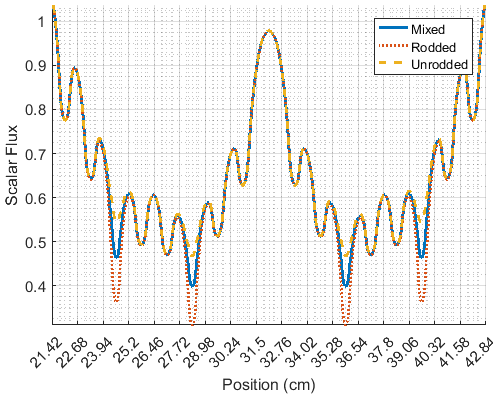
\includegraphics[width=0.8\textwidth]{../figs/1dmoc-50mix-fixedscat-scalflux7.png}
    \caption{Group 7 scalar flux comparisons for a fixed fission and scattering source calculation}\label{f:1dmoc-fixed-50-scalflux7}
\end{figure}

Figure \ref{f:1dmoc-fixed-50-scalflux7} shows the scalar flux resulting from these three calculations.  The most important thing to note in this data is that the effects of the rod are very local in the MOC calculation.  Moving through the rodded pin cell, the rodded, unrodded, and mixed cases have converged back to the same shape by the time the edge of the pin cell is reached.  This indicates that whatever treatment is used for the partially rodded cell likely does not need to worry about interference between neighboring rods because the effects are so localized.

\begin{figure}[h]
    \centering
    \subfigure[Group 1]{
        \centering
        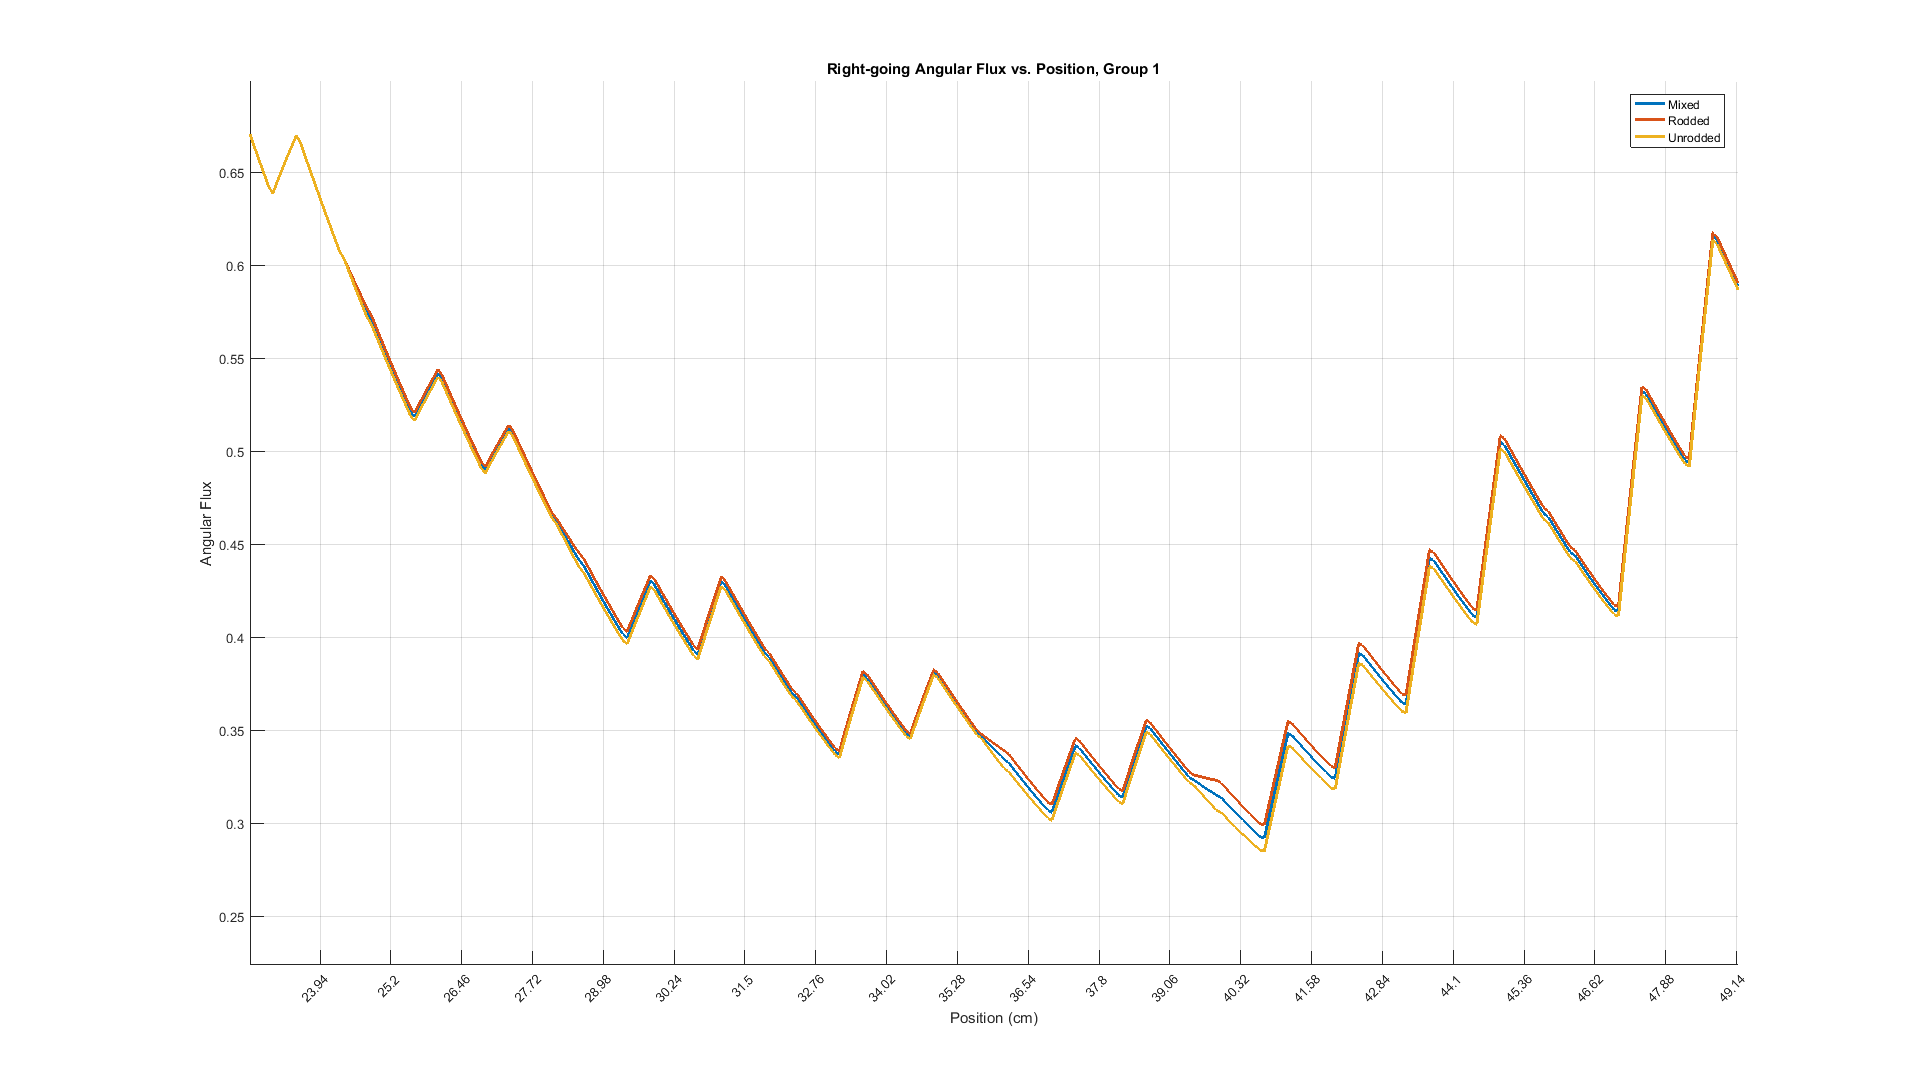
\includegraphics[width=0.45\textwidth]{../figs/1dmoc-50mix-fixedscat-angflux1.png}
        \label{f:1dmoc-fixed-50-angflux1}
    }
    ~
    \subfigure[Group 7]{
        \centering
        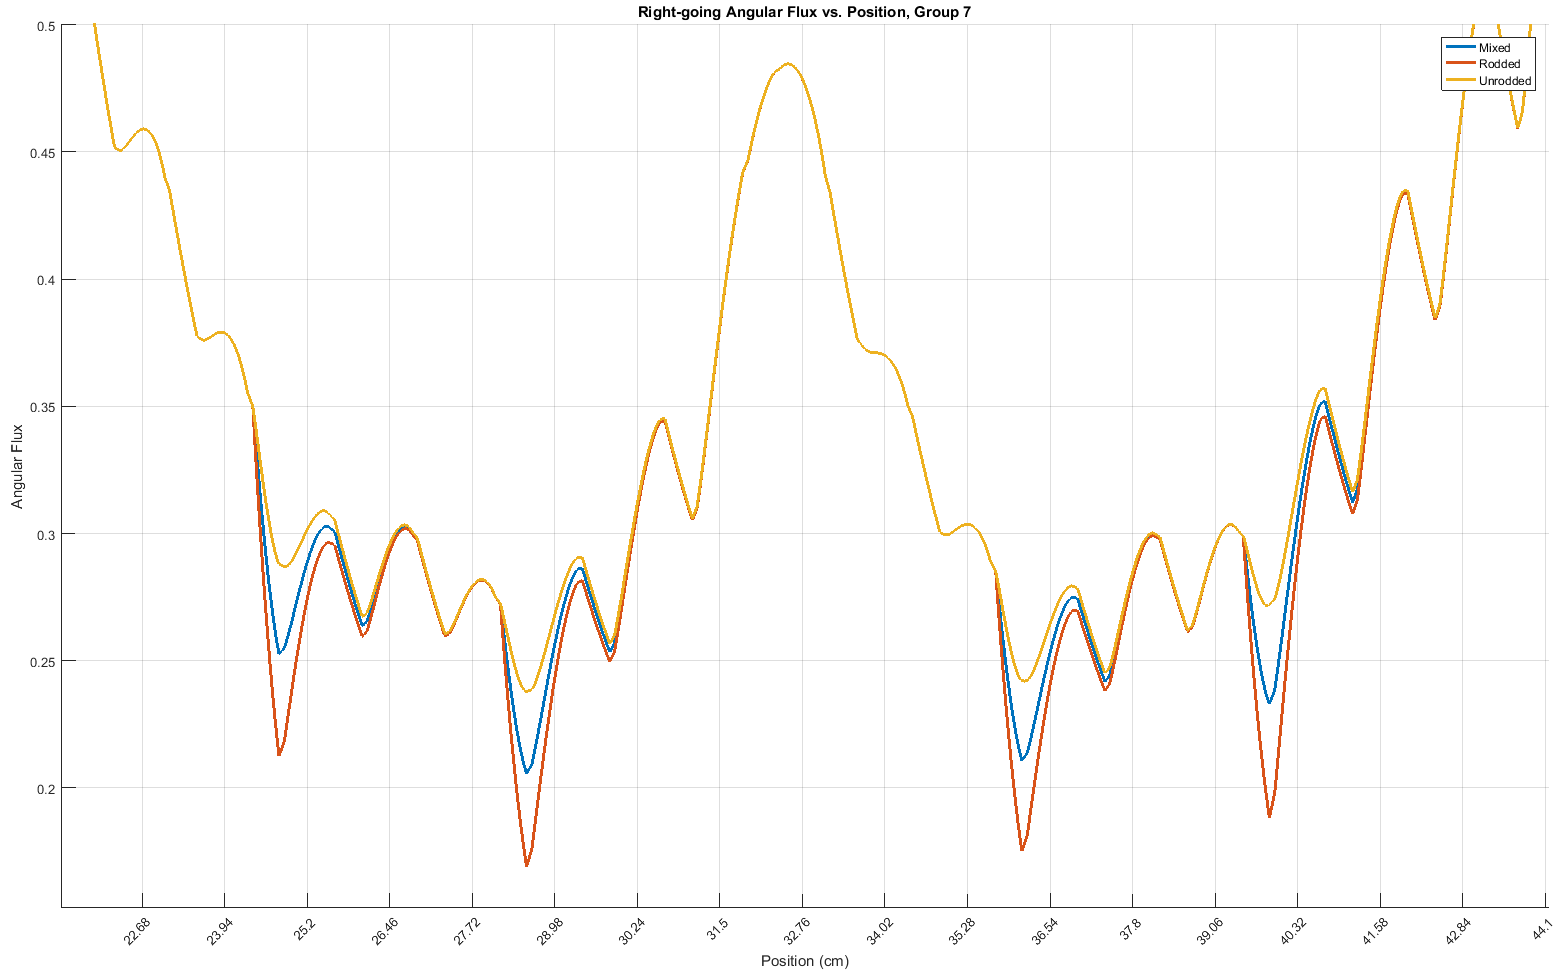
\includegraphics[width=0.45\textwidth]{../figs/1dmoc-50mix-fixedscat-angflux7.png}
        \label{f:1dmoc-fixed-50-angflux7}
    }
    \caption{Angular flux comparisons for a fixed fission and scattering source calculation}\label{f:1dmoc-fixed-50-angflux}
\end{figure}

Figure \ref{f:1dmoc-fixed-50-angflux} shows the right-going angular flux in groups 1 (fast) and group 7 (thermal).  The group 7 angular flux behaves similarly to the group 7 scalar flux in that the effects are localized around each rod.  The three different angular flux shapes are still somewhat different at the edge of the neighboring pin cell, but have pretty much converged upon reaching the clad and fuel.  The reason for this is that the mean free path of thermal neutrons is small.  The total group 7 cross-section in the moderator is about 2.65 cm$^{-1}$, which corresponds to a mean free path of about 0.38 cm, which is less than one third of the pin pitch for a typical PWR.  Because of this, the differences between the rodded and unrodded cases are washed out quickly if the source distribution is kept the same between the two calculations.

The same cannot be said for the fast flux.  The mean free path of the fast flux is about 6.3 cm, which is the width of five pin cells.  Thus, it can be seen that each of the control rods after the first builds on the effects of the previous control rod.  While the fast flux does not have a significant impact on the fission source distribution, it does impact the scattering source distribution, which is not shown in these results.

\subsubsection{Fixed Fission Source}

The second set of calculations that was performed used a fixed fission source, but allowed the scattering source to fully converge for each calculation.  As in the previous section, an eigenvalue calculation was completed using partially rodded cross-sections.  This was done for 25\%, 50\%, and 75\% rodded cases.  For each case, a fixed fission source calculation was done with the fully rodded and fully unrodded cross-sections.  This time, multiple iterations were allowed for each material to converge the scattering source.  This allows us to see the effects of the rod on the scattering source distribution without worrying about changes in the eigenvalue and fission source distribution.

\begin{figure}[h]
  \centering
  \subfigure[25\% Mixture]{
    \centering
    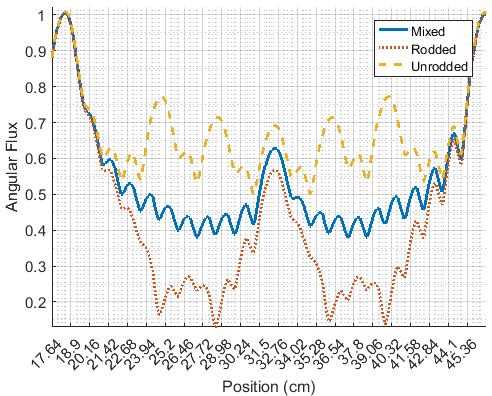
\includegraphics[width=0.45\textwidth]{../figs/1dmoc-25mix-angflux7.png}
    \label{f:1dmoc-25-angflux7}
  }
  ~
  \subfigure[50\% Mixture]{
    \centering
    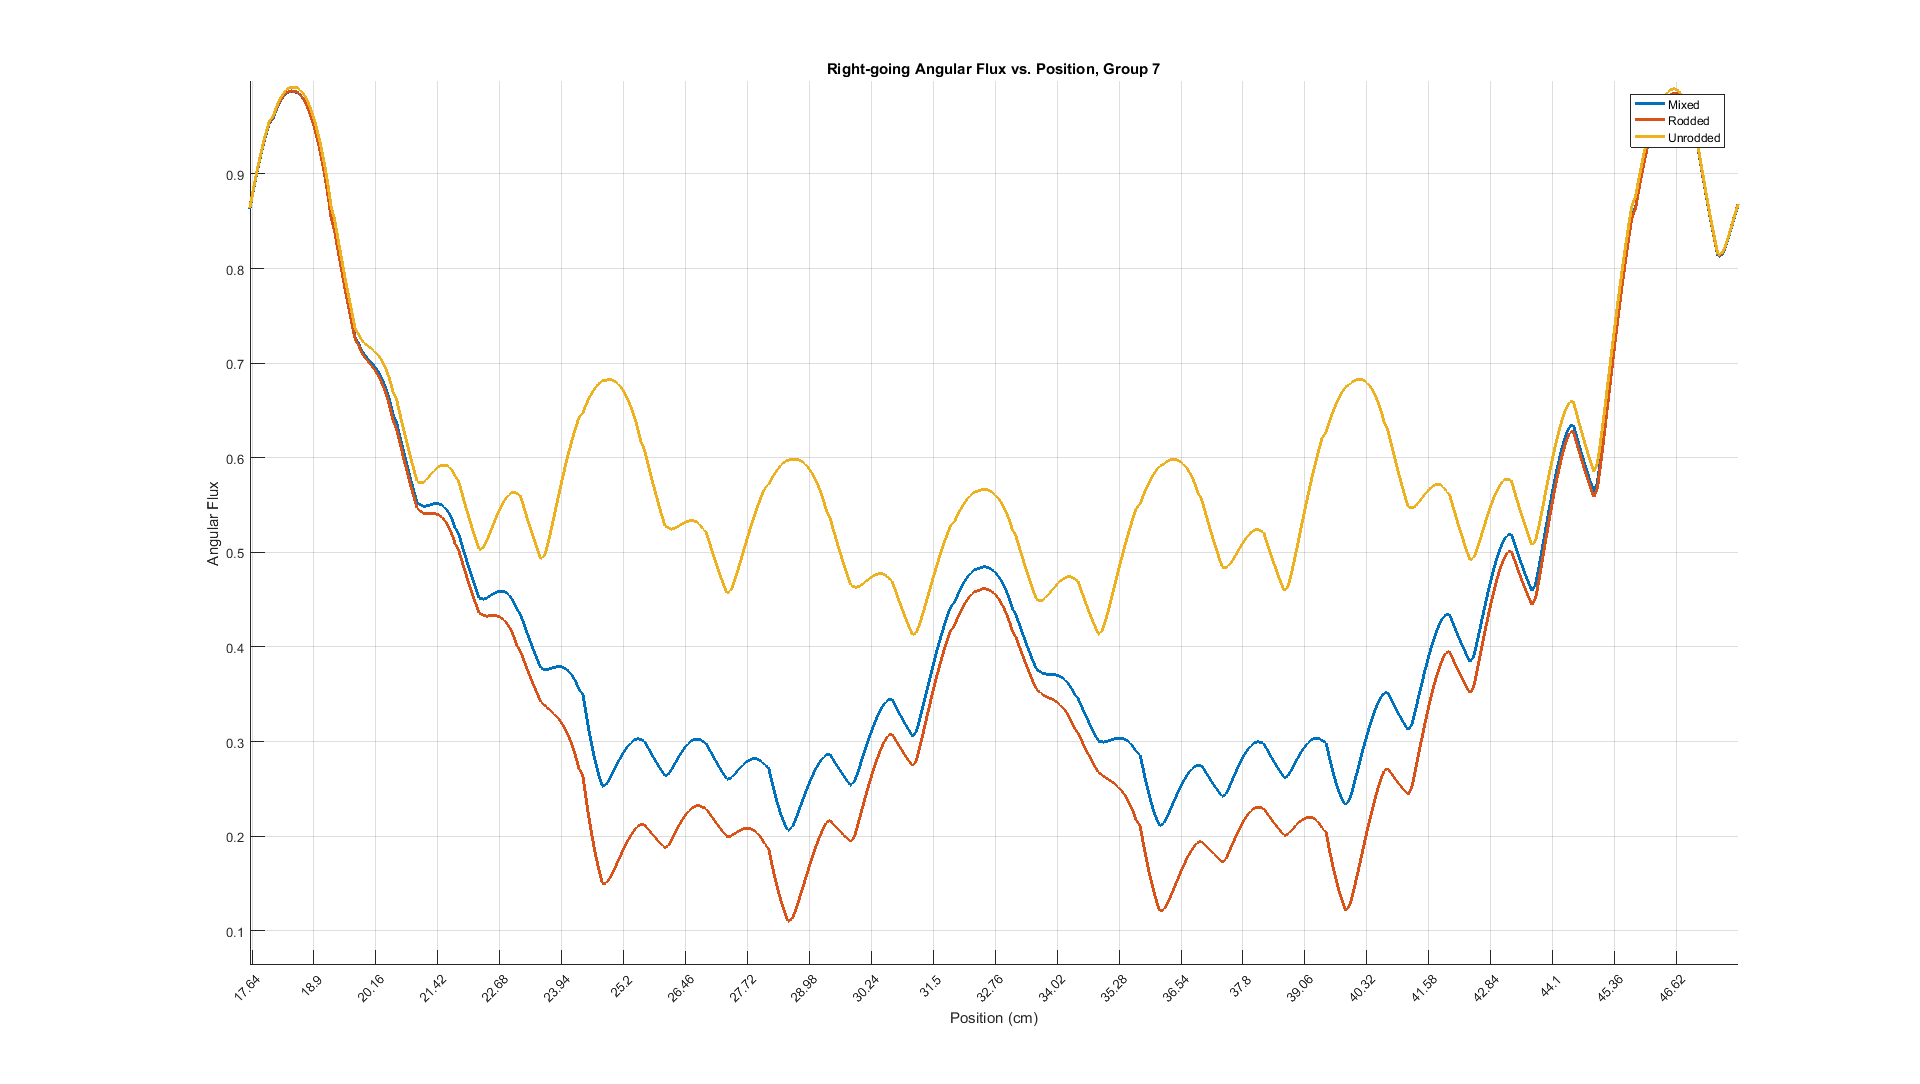
\includegraphics[width=0.45\textwidth]{../figs/1dmoc-50mix-angflux7.png}
    \label{f:1dmoc-50-angflux7}
  }
  ~
  \subfigure[75\% Mixture]{
    \centering
    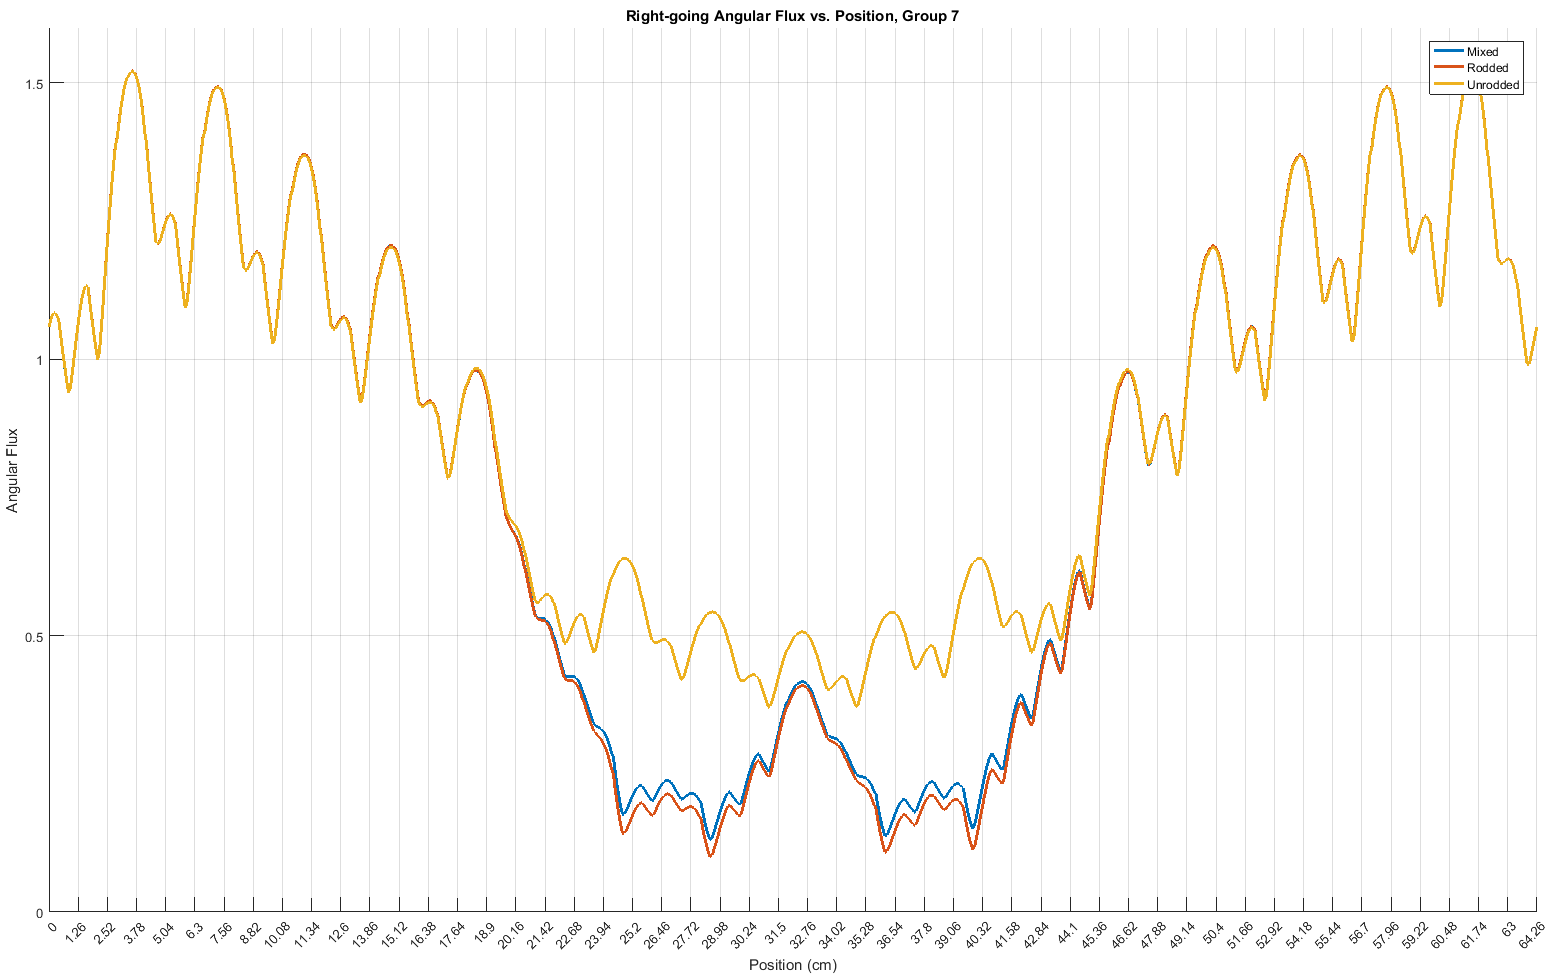
\includegraphics[width=0.45\textwidth]{../figs/1dmoc-75mix-angflux7.png}
    \label{f:1dmoc-75-angflux7}
  }
  \caption{Group 7 angular flux comparisons for 25\% and 75\% mixtures}\label{f:1dmoc-angflux7}
\end{figure}

Figure \ref{f:1dmoc-angflux7} shows the group 7 angular flux comparisons for each of the three mixtures.  We immediately see that for each of them, the angular flux for the mixture is closer to the rodded result than the unrodded result than what might be expected based on the volume fraction of the rod.  For example, comparing Figures \ref{f:1dmoc-50-angflux7} and \ref{f:1dmoc-fixed-50-angflux7} shows that the angular flux is much closer to the rodded solution than when the scattering source was fixed, despite the small mean free path of thermal neutrons.  Figure \ref{f:1dmoc-angflux1} shows the same comparisons for the group 1 angular flux.  While the difference in magnitude between each of the three cases is small for any mixture, the long mean free path means that these differences get spread out over a larger area.  This changes the shape of the scattering source for the thermal groups, which then has a more widespread effect on the the scalar flux distribution.  It should be noted as well that all angular flux plots shown here are for the flattest polar angle.  Since the steeper angles travel through more material in each region, the differences between them go away more quickly.  Thus, the angle shown in these plots is the one having the largest impact on the solution.

\begin{figure}[h]
  \centering
  \subfigure[25\% Mixture]{
    \centering
    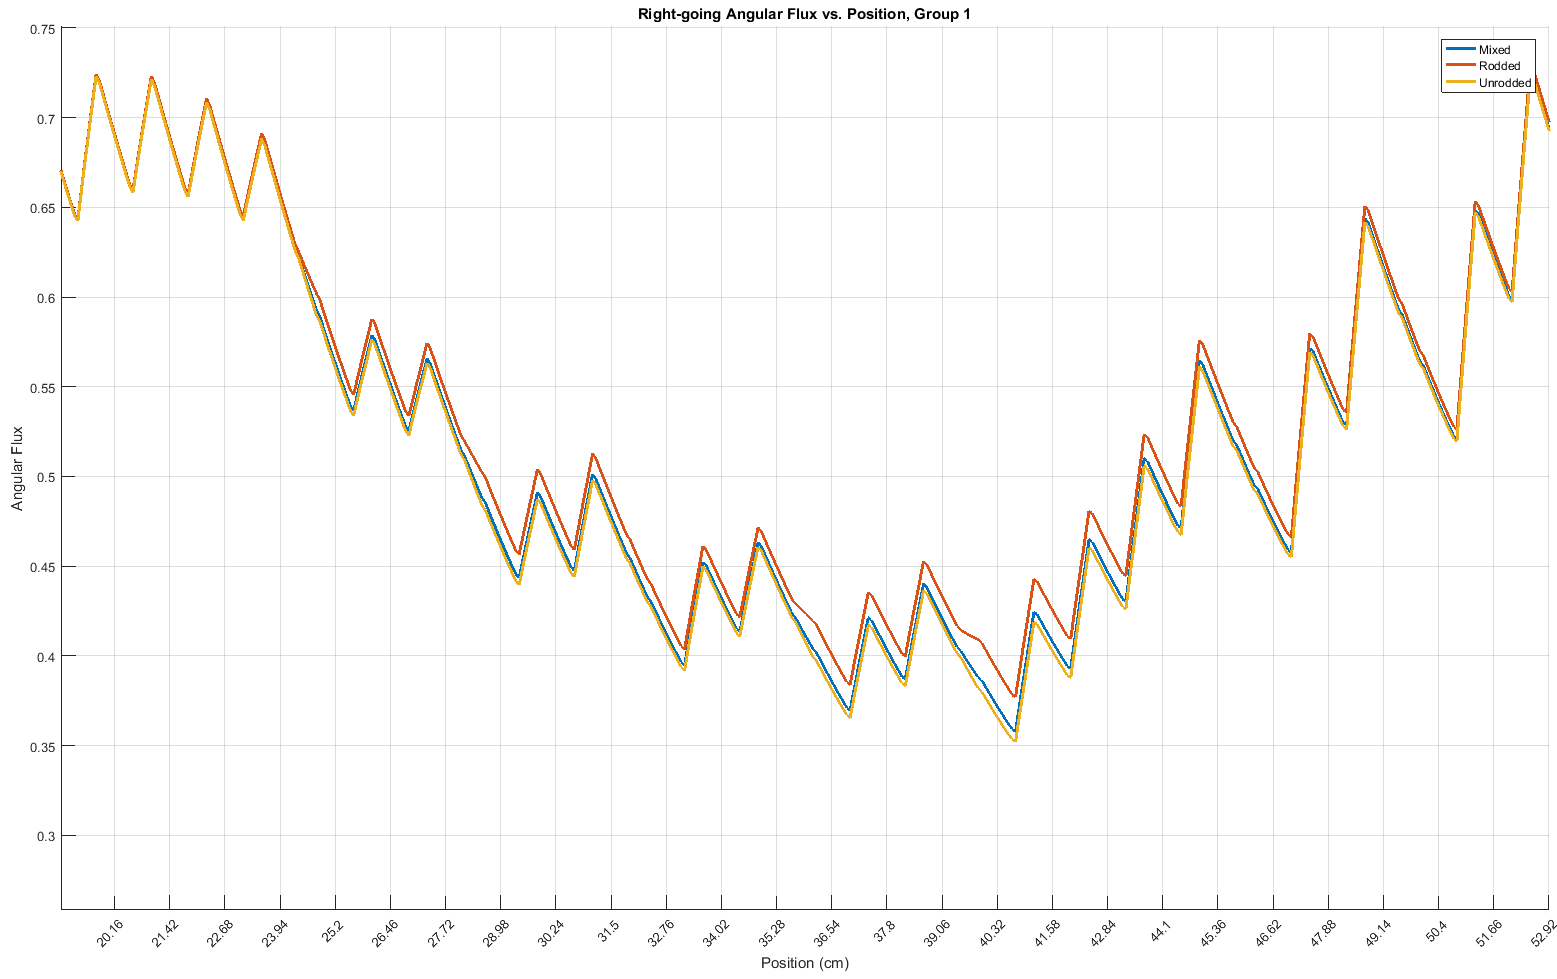
\includegraphics[width=0.45\textwidth]{../figs/1dmoc-25mix-angflux1.png}
    \label{f:1dmoc-25-angflux1}
  }
  ~
  \subfigure[50\% Mixture]{
    \centering
    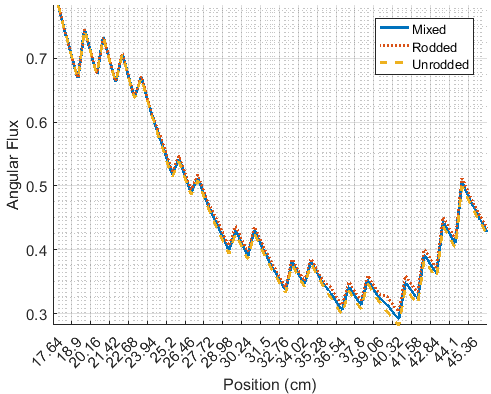
\includegraphics[width=0.45\textwidth]{../figs/1dmoc-50mix-angflux1.png}
    \label{f:1dmoc-50-angflux1}
  }
  ~
  \subfigure[75\% Mixture]{
    \centering
    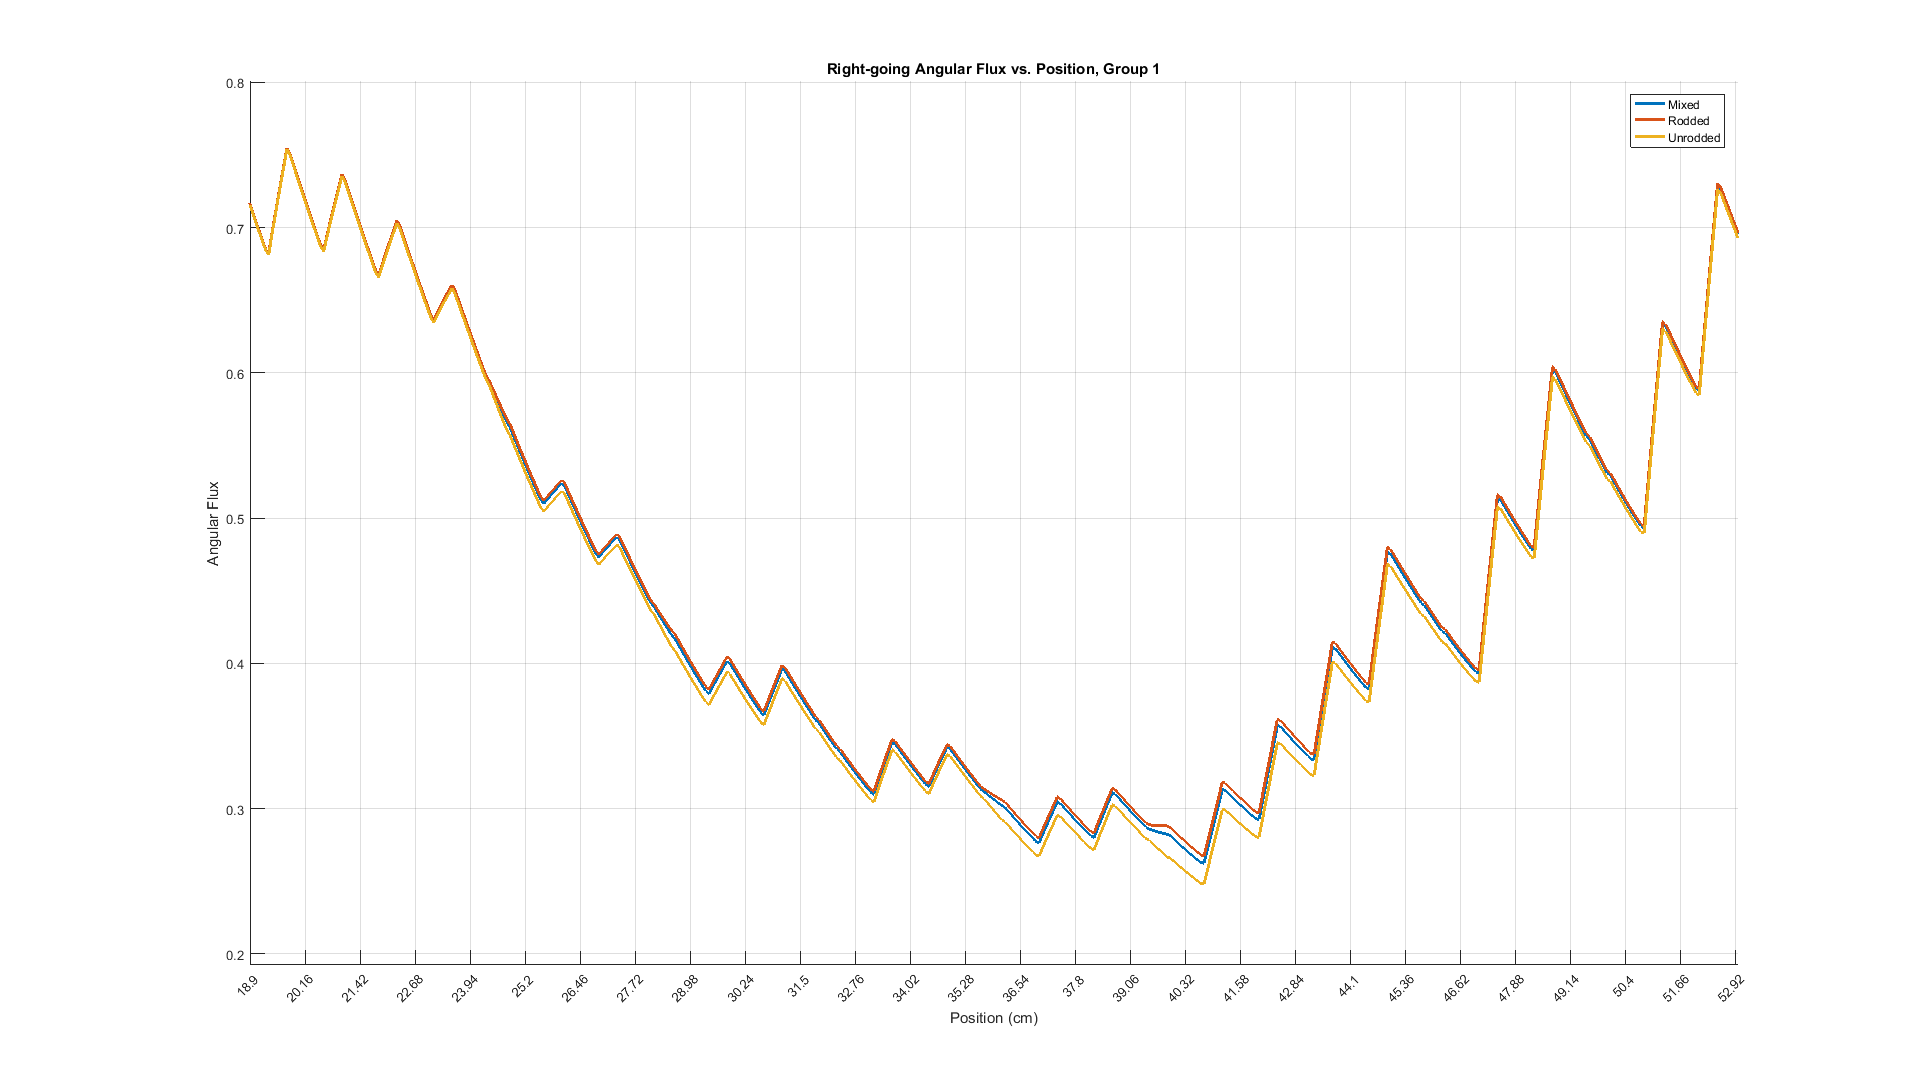
\includegraphics[width=0.45\textwidth]{../figs/1dmoc-75mix-angflux1.png}
    \label{f:1dmoc-75-angflux1}
  }
  \caption{Group 1 angular flux comparisons for 25\% and 75\% mixtures}\label{f:1dmoc-angflux1}
\end{figure}

\subsection{Sub-Ray MOC Method Description}

The 1D MOC results tells us that the effects of changing the rodded cross-section has pretty local effects on the flux itself, but the source distribution that results from these small changes in the flux then leads to significant differences in the results.  To address this, a new ``sub-ray'' MOC method will be developed.  Currently, the angular flux resulting from MPACT's MOC calculations for a partially rodded plane are simply the results of a regular MOC calculation on volume-homogenized cross-sections.  The new method will calculate two separate angular fluxes using the heterogeneous cross-sections, then combine the angular fluxes instead of the cross-sections.  This should provide a more accurate result for the scalar flux calculation, which will in turn improve the source calculations in the upcoming iterations as well.

This method will still make use of the sub-plane scheme for the CMFD and SP$_3$ calculations.  As before, sub-planes will allows the homogenized meshes to capture the axial shape of the flux.  However, they will also be beneficial to the MOC solver as well.  The rodded portion of the MOC plane will generally have a faster spectrum than the unrodded region due to absorption and a weaker ability to thermalize neutrons compared to the moderator.  Thus, two difference sources must be used in the sub-ray MOC calculations in addition to heterogeneous cross-sections.  The sub-plane scheme will provide a way to calculate those sources in the partially rodded regions.

It is clear that this method should improve the results of the calculation.  However, one of the most important outcomes of this must be that the increased computational expense must be low, otherwise there are other decusping methods that could be used, such as simply refining the axial mesh.  A single 2D assembly in MPACT (VERA Problem 2a) has 715,675 ray segments.  With a ray spacing of 0.05 cm and 16 azimuthal angles, these segments should be close to uniformly distributed amongst the 289 pin cells in the problem.  This gives an average number of segments of about 2,475 segments per pin.  For a partially rodded pin cell, we can assume that every segment in that pin cell will have two sub-rays, effectively doubling the number of segments for that pin cell.  A typical PWR such as Watts Bar has control rods in 24 positions in the lattice, so this gives a total number of segments of about 775,000 segments for a 2D assembly, or an increase of about 8\% over the original total.  Furthermore, while this is likely an accurate estimate of the increase in calculations, the actual runtime increase should be less than this.  Because the sub-rays are not actually distinct ray segments and share length and angle data, a good implementation of this method should be quite efficient in performing the extra calculations, as mentioned in section \ref{sss:2d1dMOCsweepAlgorithm} concerning the Jacobi scattering source MOC sweeping algorithm.

An execution plan was developed to map out the activities required to complete the sub-ray MOC development and implementation in MPACT.  This plan is shown in Table \ref{t:subrayExecutionPlan}

\begin{table}[h]
  \centering
  \caption{Execution plan for sub-ray MOC development and implementation}\label{t:subrayExecutionPlan}
  \begin{tabular}{|c|c|c|}\toprule
    Task & Description & Target Date \\\midrule
    1 & Analysis of cross-section and source effects on angular flux & 10/2016 \\\midrule
    2 & Development of sub-ray MOC method & 12/2016 \\\midrule
    3 & Prototype of method in 1D MOC code & 03/2017 \\\midrule
    4 & Implementation of method in MPACT & 06/2017 \\\midrule
    5 & Testing on VERA Problem 4, 5, 9 & 08/2017 \\\bottomrule
  \end{tabular}
\end{table}